% Chapter 4
\chapter{Análisis} % Main chapter title
\label{Chapter4} % Change X to a consecutive number; for referencing this chapter elsewhere, use \ref{ChapterX}

Este capítulo contiene un análisis de las diversas aplicaciones que tienen los dispositivos IoT, además se abordan las técnicas y modelos necesarios para diseñar un sistema que brinde servicio a estos dispositivos. Se comienza con una breve descripción de la red 5G y el papel que los dispositivos IoT tienen en esta. Posteriormente se profundiza en el caso de uso mMTC, donde se mencionan los escenarios más comunes de implementación, su clasificación y sus características. Se revisa también el estándar actual (NB-IoT\footnote{ Muchos\ de\ los\ modelos\ aqu\textrm{í}\ propuestos\ est\textrm{á}n\ basados\ en\ trabajos\ de\ la\ 3GPP,\ como\ se\ revis\textrm{ó}\ en\ el Capítulo II,\ la\ 3GPP,\ es\ una\ organizaci\textrm{ó}n\ que\ est\textrm{á}\ respaldada\ por\ organismos\ alrededor\ de\ todo\ el\ mundo,\ adem\textrm{á}s\ de\ que\ se\ trata\ del\ grupo\ que\ estandariza\ tecnolog\textrm{í}as\ como\ LTE-M\ y\ NB-IoT,\ de\ manera\ que\ es\ una\ indudable\ referencia\ en\ su\ ahora\ inmersi\textrm{ó}n\ en\ la\ estandarizaci\textrm{ó}n\ de\ 5G.}) que se ha seleccionado como una de las tecnologías que brindará servicio a los dispositivos IoT en la red 5G. \newline

Por último, se presentan los modelos que fueron usados para caracterizar el despliegue, la condición del canal y la generación de tráfico de comunicaciones de tipo máquina. Se presenta también una propuesta de técnica de acceso múltiple al medio no ortogonal (NOMA), que permitiría a la tecnología NB-IoT brindar servicio a más dispositivos IoT usando agrupamientos \textit{(clustering)}.

%----------------------------------------------------------------------------------------
%	SECTION 
%----------------------------------------------------------------------------------------

\section{Redes 5G/IoT}

El Internet de las cosas (IoT) tendrá un importante papel en las redes 5G. La actual red celular LTE (4G) no está diseñada para satisfacer las demandas de conectividad de múltiples dispositivos, velocidad de datos, calidad de servicio (QoS) de baja latencia y de eficiencia energética. Para abordar estos desafíos, 5G contempló a IoT como uno de sus pilares \parencite{Chetri2020}. \newline


%----------------------------------------------------------------------------------------
%	SECTION 
%----------------------------------------------------------------------------------------

\section{Clasificación y análisis de los ámbitos de IoT}

Se tomó como referencia el trabajo realizado en \parencite{NetTrafficIoT} como una guía de los servicios que se espera los nodos IoT brinden en un futuro próximo. Los servicios se presentan en 8 dominios: edificios inteligentes y vivienda (\textit{Smart buildings and living}), cuidado de la salud inteligente (\textit{Smart healthcare}), medio ambiente inteligente (\textit{Smart environment}), ciudades inteligentes (\textit{Smart city}), energía inteligente (\textit{Smart energy}), transporte y movilidad  inteligentes (\textit{Smart transport and mobility}), fabricación y venta inteligentes (\textit{Smart manufacturing and retail}), agricultura inteligente (\textit{Smart agriculture}). Para cada uno de los dominios se especifican aplicaciones típicas que se podrían encontrar, sus características de tráfico y las tecnologías de red más adecuadas para darles servicio entre otras cosas.\newline

La primera parte del análisis correspondió a la selección de los dominios que resultasen adecuados para el sistema que se diseñó. Los dominios seleccionados fueron aquellos que se acoplan primordialmente es una red de área amplia de bajo consumo (LPWAN, \textit{Low Power Wide Area Network}). Por el contrario, algunas de las aplicaciones en los dominios antes mencionados están pensadas para redes con tecnologías como RFID, \textit{Bluetooth }o \textit{ZigBee }. A continuación se presenta la caracterización de cada uno de los dominios que en \parencite{NetTrafficIoT} se consideran viables para redes LPWAN.

\subsection{Ciudades inteligentes \textit{(Smart Cities)}:}

Con la rápida concentración de la poblacion en zonas urbanas, se ha convertido en una prioridad la reducción del uso de recursos públicos, así como la reducción de costos de operación del día a día de una ciudad. Las aplicaciones en este dominio tratan justamente de abordar estos problemas y los servicios que brindan son bastante variados. Los ejemplos van desde el control de luminarias hasta el manejo de desechos, estos y otros  pueden encontrarse en la \textit{Tabla~\ref{tab:smartcity}}, acompañados de más información tal como la caracterización de su tráfico y su demanda de QoS.

\begin{table}
\caption{Características de las aplicaciones de Ciudades Inteligentes}
\label{tab:smartcity}
\centering
\begin{tabular}{*{5}{m{3cm}}}\\
\textbf{\textit{Servicio}} & \textbf{\textit{Tamaño de red}} & \textbf{\textit{Tasa de tráfico}} & \textbf{\textit{Demanda de QoS}} & \textbf{\textit{Fuente de energía}} \\ \hline \hline
\textit{Monitoreo del consumo de agua y electricidad en la ciudad} & \footnotesize{Media a grande, cientos a miles de dispositivos} & \footnotesize{Periódico, 1 msj cada 10 min por dispositivo} & \footnotesize{Baja, tolerante al retardo 1 min} & \footnotesize{Alimentado por la red eléctrica/ autoalimentado} \\ \hline
\textit{Control de iluminación} & \footnotesize{Grande, miles de dispositivos} & \footnotesize{Aleatorio, poco frecuente} & \footnotesize{Media, tolerante al retardo 15 seg} & \footnotesize{Alimentado por la red eléctrica }\\ \hline
\textit{Vigilancia de estacionamientos} & \footnotesize{Grande, miles de dispositivos} & \footnotesize{Aleatorio, poco frecuente} & \footnotesize{Media, tolerante al retardo 10 seg} & \footnotesize{Alimentado por batería }\\ \hline
\textit{Control del tráfico} & \footnotesize{Grande, miles de dispositivos} & \footnotesize{Periódico, 1 msj cada 10 min por dispositivo, aleatorio para alarmas} & \footnotesize{Media, tolerante al retardo 15 seg, alta para alarmas} & \footnotesize{Alimentado por batería} \\ \hline
\textit{Mantenimiento de deshechos} & \footnotesize{Grande, miles de dispositivos} & \footnotesize{Aleatorio, poco frecuente} & \footnotesize{Media, tolerante al retardo 30 seg} & \footnotesize{Alimentado por batería }\\ \hline
\textit{Monitoreo de condiciones urbanas} & \footnotesize{Media a grande, cientos a miles de dispositivos} & \footnotesize{Periódico, 1 msj cada 15 min por dispositivo, aleatorio para alarmas} & \footnotesize{Media, tolerante al retardo 30 seg, alta para alarmas} & \footnotesize{Alimentado por batería }\\ \hline
\textit{Monitoreo de la salud estructural de edificios} & \footnotesize{Media a grande, cientos a miles de dispositivos} & \footnotesize{Periódico, 1 msj cada 15 min por dispositivo, aleatorio para alarmas} & \footnotesize{Media, tolerante al retardo 30 seg, alta para alarmas} & \footnotesize{Alimentado por batería} \\ 
\end{tabular}
\end{table}

\subsection{Ambiente inteligente \textit{(Smart Environment)}}

Este dominio comprende las aplicaciones que se encargan de monitorear lo que ocurre a nuestro alrededor. Una de las ventajas de monitorear el ambiente es el poder reaccionar con antelación a eventos que de otra forma causarían muchos daños. En la \textit{Tabla~\ref{tab:smartenv}} podemos encontrar la caracterización de las aplicaciones consideradas en \parencite{NetTrafficIoT} para Ambiente Inteligente.

\begin{table}
\caption{Características de las aplicaciones de Ambiente Inteligente}
\label{tab:smartenv}
\centering
\begin{tabular}{*{5}{m{3cm}}} \\ 
\textbf{\textit{Servicio}} & \textbf{Tamaño de red} & \textbf{Tasa de tráfico} & \textbf{Demanda de QoS} & \textbf{Fuente de energía} \\ \hline \hline
\textit{Detección de incendios forestales}  & \footnotesize{ Media a grande, cientos a miles de dispositivos } & \footnotesize{ Aleatorio, poco frecuente } & \footnotesize{ Media, tolerante al retardo 15 seg } & \footnotesize{ Alimentado por batería } \\ \hline 
\textit{Detección de terremotos}  & \footnotesize{ Media a grande, cientos a miles de dispositivos } & \footnotesize{ Aleatorio, poco frecuente } & \footnotesize{ Alta, tolerante al retardo 5 seg } & \footnotesize{ Alimentado por batería } \\ \hline 
\textit{Detección de Tsunamis}  & \footnotesize{ Media a grande, cientos a miles de dispositivos } & \footnotesize{ Aleatorio, poco frecuente } & \footnotesize{ Alta, tolerante al retardo 5 seg } & \footnotesize{ Alimentado por batería } \\ \hline 
\textit{Detección de derrumbes y avalanchas}  & \footnotesize{ Media a grande, cientos a miles de dispositivos } & \footnotesize{ Aleatorio, poco frecuente } & \footnotesize{ Alta, tolerante al retardo 5 seg } & \footnotesize{ Alimentado por batería } \\ \hline 
\textit{Monitoreo de actividad volcánica}  & \footnotesize{ Pequeña, 10s de dispositivos } & \footnotesize{ Aleatorio, poco frecuente } & \footnotesize{ Alta, tolerante al retardo 5 seg } & \footnotesize{ Alimentado por batería } \\ \hline 
\textit{Monitoreo de la contaminación del aire } & \footnotesize{ Media a grande, cientos a miles de dispositivos } & \footnotesize{ Periódico, 1 msj cada 15 min por dispositivo } & \footnotesize{ Media, tolerante al retardo 15 seg } & \footnotesize{ Alimentado por batería } \\ \hline 
\textit{Rastreo de vida salvaje.}  & \footnotesize{ Media, cientos de dispositivos } & \footnotesize{ Periódico, 1 msj cada 30 min por dispositivo } & \footnotesize{ Baja, tolerante a unas horas } & \footnotesize{ Alimentado por batería } \\ 
\end{tabular}
\end{table}

\subsection{Energía inteligente \textit{(Smart Energy)}:}

El dominio de Energía Inteligente (\textit{Smart Energy}) contempla mejoras en la distribución y el consumo de fuentes de energía o recursos vitales, tales como la electricidad, el gas y el agua. Actualmente el foco de atención está en la electricidad ya que existe una tendencia más marcada hacia su ahorro y la utilización de fuentes renovables. \newline

Los nodos de IoT que operen dentro de este dominio podrían monitorear las condiciones cambiantes de la red eléctrica, para posteriormente generar una reconfiguración apropiada del servicio. En la \textit{Tabla~\ref{tab:smartenergy}} podemos encontrar la caracterización descrita en \parencite{NetTrafficIoT} para distintas aplicaciones de Energía Inteligente.

\begin{table}
\caption{Características de las aplicaciones de Energía Inteligente}
\label{tab:smartenergy}
\centering
\begin{tabular}{*{5}{m{3cm}}}  \\  
\textbf{\textit{Servicio}} & \textbf{Tamaño de red} & \textbf{Tasa de tráfico} & \textbf{Demanda de QoS} & \textbf{Fuente de energía} \\ \hline \hline
\textit{Medición inteligente}  & \footnotesize{ Media a grande, 1 dispositivo por hogar } & \footnotesize{ Periódico, 1 msj cada 15 min por dispositivo } & \footnotesize{ Media, tolerante al retardo 15 seg } & \footnotesize{ Alimentado por la red eléctrica/ Baterías } \\ \hline 
\textit{Gestión de activos}  & \footnotesize{ Media a grande, cientos a miles de dispositivos } & \footnotesize{ Periódico, 1 msj cada 15 min por dispositivo } & \footnotesize{ Media, tolerante al retardo 15 seg } & \footnotesize{ Alimentado por la red eléctrica/ Baterías } \\ \hline 
\textit{Detección de interrupciones en el servicio } & \footnotesize{ Media a grande, 1 dispositivo por hogar } & \footnotesize{ Aleatorio, poco frecuente } & \footnotesize{ Alta, tiempo real } & \footnotesize{ Alimentado por la red eléctrica/ Baterías } \\ 
\end{tabular}
\end{table}

\subsection{Transporte y movilidad inteligentes \textit{(Smart Transport and Mobility)}:}

Tanto el crecimiento urbano como el crecimiento de las fuentes de transporte de pasajeros y de mercancías, han creado la necesidad de administrar más eficientemente la movilidad en ciudades y carreteras. \newline

El objetivo de aplicaciones IoT en el dominio de Transporte y movilidad inteligentes (\textit{ (Smart Transport and Mobility)}) es ayudar a resolver el problema de movilidad tanto de pasajeros como de mercancías, haciéndolo más rápido, más barato y más seguro. En la \textit{Tabla~\ref{tab:smartrans}} se encuentra la caracterización presentada en \parencite{NetTrafficIoT} para distintas aplicaciones de este dominio.\newline

El análisis de las aplicaciones seleccionadas, provenientes de distintos dominios, se presenta en la siguiente sección.

\begin{table}
\caption{Características de las aplicaciones de Transporte y Movilidad inteligentes}
\label{tab:smartrans}
\centering
\begin{tabular}{*{5}{m{3cm}}}\\ 
\textit{Servicio} & Tamaño de red & Tasa de tráfico & Demanda de QoS & Fuente de energía \\ \hline \hline
\textit{Automatización de vehículos}  & \footnotesize{ Grande, miles de dispositivos } & \footnotesize{ Periódico, 1 msj cada 24 hrs por vehículo. } & \footnotesize{ Baja, tolerante al retardo 1 min } & \footnotesize{ Alimentado por batería del vehículo } \\ \hline 
\textit{Localización y monitoreo de vehículos}  & \footnotesize{ Grande, miles de dispositivos } & \footnotesize{ Periódico, 1 msj cada 30 seg por vehículo } & \footnotesize{ Media, tolerante al retardo 10 seg } & \footnotesize{ Alimentado por batería del vehículo } \\ \hline 
\textit{Monitoreo de la calidad del embarque}  & \footnotesize{ Media, cientos de dispositivos } & \footnotesize{ Periódico, 1 msj cada 15 min por dispositivo } & \footnotesize{ Media, tolerante al retardo 15 seg } & \footnotesize{ Alimentado por batería } \\ \hline 
\textit{Control dinámico de semáforos}  & \footnotesize{ Grande, miles de dispositivos } & \footnotesize{ Periódico, 1 msj cada min por dispositivo } & \footnotesize{ Alta, tolerante al retardo 5 seg } & \footnotesize{ Alimentado por la red eléctrica } \\ \hline 
\textit{Monitoreo de las condiciones del camino} & \footnotesize{ Grande, miles de dispositivos } & \footnotesize{ Aleatorio, poco frecuente } & \footnotesize{ Media, tolerante al retardo 30 seg } & \footnotesize{ Alimentado por batería } \\
\end{tabular}
\end{table}

%----------------------------------------------------------------------------------------
%	SECTION 
%----------------------------------------------------------------------------------------

\section{Características del escenario a implementar}\label{AppsEscenario}

Las distintas aplicaciones presentadas en la sección anterior muy seguramente se verán desplegadas en un futuro próximo en ciudades alrededor de todo el mundo. Una aserción que resulta importante es la gran cantidad de aplicaciones que se esperan para IoT \parencite{Ericsson2019}, pero en este análisis se tomaron en consideración únicamente aquellas que operan en una red LPWAN. Para estas aplicaciones, una red celular de 5G podría ser las más idónea para brindarles servicio. \newline

En las aplicaciones seleccionadas, lo primordial es tener un bajo consumo y complejidad de los dispositivos, además de una amplia cobertura y permitir una gran densidad de dispositivos \parencite{5GAmericas}. Esto contrasta con las aplicaciones más inclinadas a los casos de uso eMBB y URLLC, para las cuales lo primordial es el amplio ancho de banda disponible para las aplicaciones y una menor latencia, respectivamente.

\subsection{Análisis de las aplicaciones de IoT y selección de casos considerados}

De todos los servicios descritos en las tablas anteriores \textit{[Tabla~\ref{tab:smartcity}\ldots \ref{tab:smartrans}]}, se decidió implementar solamente un grupo diverso de aplicaciones provenientes de distintos dominios. Este grupo se seleccionó de tal manera que fuera representativo de distintos comportamientos y requerimientos de QoS. El escenario propuesto consta de los servicios de: control de iluminación, monitoreo del consumo de agua y electricidad, detección de terremotos, monitoreo de contaminación del aire, detección de interrupciones en el servicio (agua, luz, gas), control dinámico de semáforos y un último servicio que se llamó ``otros dispositivos mMTC''. Este último representó el conglomerado de todas las demás aplicaciones IoT que estarán presentes en la red y no corresponden a una de las primeras aplicaciones seleccionadas. \newline

Se decidió entonces situar la simulación en un escenario urbano macro celular (UMa) con nodos en exteriores, en el que se encontrarán todas las aplicaciones mencionadas en el párrafo anterior. El escenario urbano macro representa a zonas urbanas densamente pobladas. La elección de un escenario urbano macro celular se debió a que en este se puede experimentar una congestión producida por las  MTC y HTC más facilmente. Otra razón fue que en tal escenario se tiene presente una mayor diversidad de aplicaciones IoT, con distintas características de tráfico y requerimientos de QoS.\newline

En la \textit{Tabla~\ref{tab:appssim}} se presentan las aplicaciones IoT del escenario urbano que se implementaron.\newline

A continuación se hace una descripción de la \textit{Tabla~\ref{tab:appssim}}. Se tienen tres aplicaciones con una alta demanda de QoS, después dos con una demanda media y finalmente una con demanda baja. Las distintas demandas de QoS se traducen en diferentes tolerancias a la latencia, las cuales van desde los minutos hasta aquellas que requieren de una respuesta en el orden de segundos. Otra característica que se consideró para decidir entre las aplicaciones fue su tráfico, se trató entonces de tener nodos con distintos periodos de transmisión, por ejemplo el servicio que brindan nodos monitoreando la contaminación del aire tiene un periodo de 15 minutos, mientras que el de nodos controlando los semáforos es de 1 minuto. Existen también nodos con tasas de trasmisión aleatorias como el caso de los nodos de detección de terremotos. \newline

La decisión de agregar un servicio más (Otros dispositivos mMTC) que fuera genérico surge a raíz de la necesidad de representar en la red los dispositivos restantes con comportamientos de lo más diversos.\newline

Finalmente se consideraron también dispositivos URLLC en el simulador. Esto permitió realizar un agrupamiento de dispositivos mMTC y URLLC para que pudieran compartir recursos. Los detalles de la implementación son discutidos en los siguientes capítulos.

\begin{table}
\caption{Aplicaciones seleccionadas para la simulación}
\label{tab:appssim}
\centering
\begin{tabular}{*{5}{m{3cm}}} \\ 
\textbf{\textit{Servicio}} & \textbf{Tamaño de red} & \textbf{Tasa de tráfico} & \textbf{Demanda de QoS} & \textbf{Fuente de energía} \\ \hline \hline
\textit{Control de iluminación (Ciudad Inteligente)}  & \footnotesize{ Grande, miles de dispositivos } & \footnotesize{ Aleatorio, poco frecuente } & \footnotesize{ Media, tolerante al retardo 15seg } & \footnotesize{ Alimentado por la red eléctrica } \\ \hline 
\textit{Monitoreo del consumo de agua y electricidad en la ciudad (Ciudad Inteligente)}  & \footnotesize{ Media a grande, cientos a miles de dispositivos } & \footnotesize{ Periódico, 1 msj cada 10 min por dispositivo } & \footnotesize{ Baja, tolerante al retardo 1min } & \footnotesize{ Alimentado por la red eléctrica/ autoalimentado } \\ \hline 
\textit{Detección de terremotos (Ambiente Inteligente)}  & \footnotesize{ Media a grande, cientos a miles de dispositivos } & \footnotesize{ Aleatorio, poco frecuente } & \footnotesize{ Alta, tolerante al retardo 3seg } & \footnotesize{ Alimentado por batería } \\ \hline 
\textit{Monitoreo de contaminación del aire (Ambiente Inteligente) } & \footnotesize{ Media a grande, cientos a miles de dispositivos } & \footnotesize{ Periódico, 1 msj cada 15 min por dispositivo } & \footnotesize{ Media, tolerante al retardo 15seg } & \footnotesize{ Alimentado por batería } \\ \hline 
\textit{Control dinámico de semáforos (Transporte y Movilidad Inteligentes)} & \footnotesize{ Grande, miles de dispositivos } & \footnotesize{ Periódico, 1 msj cada min por dispositivo } & \footnotesize{ Alta, tolerante al retardo 5seg } & \footnotesize{ Alimentado por la red } \\ \hline 
\textit{Otros dispositivos mMTC}  & \footnotesize{ Grande, miles de dispositivos } & \footnotesize{ Aleatorio, poco frecuente } & \footnotesize{ Alta, tolerante al retardo 5seg } & \footnotesize{ Alimentado por batería } \\ 
\end{tabular}
\end{table}


\subsection{Análisis de las tecnologías para IoT y selección de casos considerados}

NB-IoT y LTE-M (\textit{LTE for MTC}) son dos tecnologías LPWA desarrolladas para aplicaciones IoT. Ambas tecnologías contemplan comunicaciones celulares con un ancho de banda bajo, y conectan dispositivos que necesitan transmitir pequeñas cantidades de datos, a bajo coste. Debido a que se espera que NB-IoT y LTE-M cumplan con los requerimientos LPWAN del estándar 5G, 3GPP indicó a ITU-R que ambas tecnologías formarán parte del estándar. Estas tecnologías coexistirán con los demás componentes de 5G NR que en conjunto brindarán servicio a los distintos casos de uso. Esto convierte a NB-IoT y LTE-M parte de 5G \parencite{EricssonAB2016}. De entre las dos tecnologías, la que mejor satisface los requerimientos de las aplicaciones seleccionadas en la sección anterior es NB-IoT como se desarrolla a continuación.\newline

Las redes de largo alcance LPWAN utilizan tecnología capaz de transferir mensajes a decenas de kilómetros de distancia y cubrir una amplia área. Son redes especializadas en interconectar dispositivos en ambientes restringidos, de difícil acceso o que simplemente buscan reducir el consumo de energía en estos, manteniendo un bajo costo y complejidad. Por lo tanto se concentran en un eficiente consumo de la energía y una cobertura amplia \parencite{NetTrafficIoT}. Esto se acopla bastante bien a lo que requieren los nodos de IoT pertenecientes a las aplicaciones seleccionadas en la sección anterior. \newline

Las tecnologías que darán servicio a dispositivos IoT son entonces:

\begin{enumerate}
    \item \textit{\underbar{eMTC (enhanced Machine Type Communication:)}} Forma parte de la familia LTE-M y es una evolución de LTE optimizada para IoT. Se desarrolló con el objetivo de una eficiencia energética.
    \item \textit{\underbar{NB-IoT (Narrow-Band Internet of Things:)}} fue estandarizado en el \textit{release }13 de 3GPP y se espera que consiga dar servicio a más dispositivos con energía limitada que eMTC. NB-IoT no requiere ningún desarrollo adicional de redes ya que se implementa en funcionalidades ya existentes de LTE \parencite{NetTrafficIoT} y en un futuro será implementado directamente en la banda de frecuencias de 5G NR [\textit{véase Figura~\ref{fig:5gnr}}] \parencite{EricssonAB2016}.
\end{enumerate}

El soporte para IoT masivo (mIoT) ya se brinda en las redes LTE de hoy con NB-IoT y eMTC. Estas tecnologías se complementan entre sí y existe una tendencia emergente de los proveedores de servicios de implementar una red común que admita ambas tecnologías. eMTC es adecuada para casos de uso que requieren un rendimiento relativamente más alto, una latencia más baja y soporte de voz, mientras que la tecnología NB-IoT es conveniente para casos de uso que toleren demoras pero requieren una cobertura extendida \parencite{EricssonAB2016}. \newline

Según \parencite{Ericsson2019} a finales de 2024, se espera que NB-IoT y eMTC representen cerca del 45 por ciento de todas las conexiones CIoT (\textit{Celullar IoT}). Además, en el futuro NB-IoT y eMTC podrán coexistir completamente en las bandas de frecuencia de 5G NR, \textit{Figura~\ref{fig:5gnr}}.\newline

\begin{figure}[th]
\centering
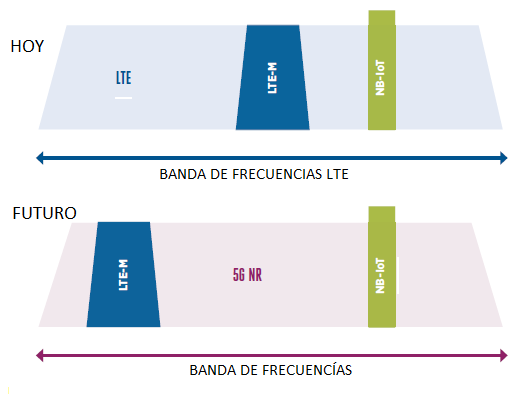
\includegraphics[scale=1]{Figures/5G NR con LTE-M y NB-IoT en banda}
\decoRule
\caption[5G NR con LTE-M y NB-IoT en banda]{5G NR con LTE-M y NB-IoT en banda}
\label{fig:5gnr}
\end{figure}

En la \textit{Tabla~\ref{tab:tecIoT}} se pueden encontrar características de estas tecnologías antes descritas, tales como la banda de frecuencia a la que operan y su tasa de transmisión. Si bien pareciera que la diferencia entre ambas tecnologías es sutil, en realidad, esta marca una clara pauta en el servicio que pueden brindar. \newline

\begin{table}
\caption{Características de las tecnologías de red para IoT en la red celular}
\label{tab:tecIoT}
\centering
\begin{tabular}{|p{0.9in}|p{0.6in}|p{0.4in}|p{0.6in}|p{0.4in}|p{0.8in}|p{1.3in}|p{0.4in}|} \\ \hline \hline
\textbf{\textit{Tecnología}} & \textbf{\textit{Banda de Frecuencia}} & \textbf{\textit{Rango}} & \textbf{\textit{Tasa de transmisión}} & \textbf{\textit{Vida de la batería}} & \textbf{\textit{Topología}} & \textbf{\textit{Estandarización}} & \textbf{\textit{Grupo}} \\ 
\textbf{NB-IoT}  & \footnotesize{ 450 MHZ -- 3.5 GHz (Espectro de 2G/3G/4G) } & \footnotesize{ 10-15 km } & \footnotesize{ 250 kbps } & \footnotesize{ 10+ años } & \footnotesize{ Estrella } & \footnotesize{ Abierta } & \footnotesize{ 3GPP } \\ \hline
\textbf{eMTC}  & \footnotesize{ 450 MHZ -- 3.5 GHz (El mismo que LTE) } & \footnotesize{ 10-15 km } & \footnotesize{ 1 Mbps } & \footnotesize{ 10+ años } & \footnotesize{ Estrella } & \footnotesize{ Abierta } & \footnotesize{ 3GPP } \\
\end{tabular}

\end{table}

En la \textit{Figura~\ref{fig:lpwa}} se puede observar otra comparación entre ambas tecnologías pero en esta ocasión se comparan las aplicaciones a las que  NB-IoT y LTE-M estarían dando servicio preferentemente. A la izquierda de la \textit{Figura~\ref{fig:lpwa}} tenemos las aplicaciones LPWAN a las que NB-IoT daría servicio. Estas aplicacioness coinciden con una menor velocidad de transferencia y mayor tolerancia a la latencia mientras que a la derecha se aglomeran las aplicaciones que requieren una comunicación de baja latencia y una mayor tasa de transmisión. A estas últimas aplicaciones les estaría dando servicio preferentemente la tecnología eMTC. \newline

Se decidió entonces concentrarse en la tecnología NB-IoT puesto que la totalidad de los servicios que se considerarán en nuestro sistema pueden situarse a la izquierda de la \textit{Figura~\ref{fig:lpwa}}, donde se presenta una mínima movilidad de los dispositivos. Por ejemplo el control de la iluminación y el control dinámico de los semáforos podríamos colocarlos en \textit{Iluminación pública y Ciudades inteligentes }respectivamente, mientras que el monitoreo de consumo energético y el de la condición del aire podrían corresponder a \textit{Medidores inteligentes}, de manera que el único servicio que se situa en los límites de la tecnología NB-IoT o del otro lado incluso es el de dispositivos URLLC. Debido a esto se seleccionó a NB-IoT como la tecnología fundamental para diseñar el simulador a la que después se agregaron mejoras propuestas en otros trabajos.  \newline


\begin{figure}[th]
\centering
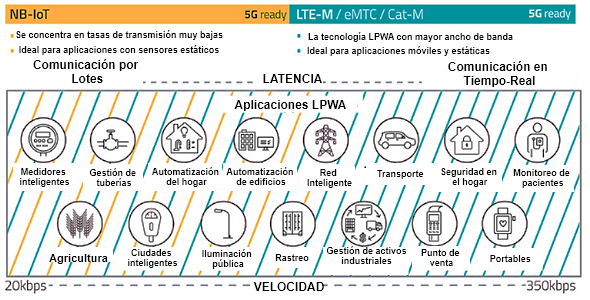
\includegraphics[scale=1]{Tecnología líder para el caso de uso LPWA}
\decoRule
\caption[Tecnologías líderes para el caso de uso LPWA]{Tecnologías líder para el caso de uso LPWA, [Fuente: https://www.iotforall.com/cellular-iot-explained-nb-iot-vs-lte-m/]}
\label{fig:lpwa}
\end{figure}


La \textit{Figura~\ref{fig:5gqos}} muestra las distintas tecnologías con las que 5G NR estaría trabajando para poder brindar servicio al amplio espectro de casos de uso de MTC \parencite{5GAmericas}. La tecnología NB-IoT podemos situarla en las frecuencias de operación baja y con un una tolerancia al retardo mayor que la mayoría de las demás tecnologías.

\begin{figure}[th]
\centering
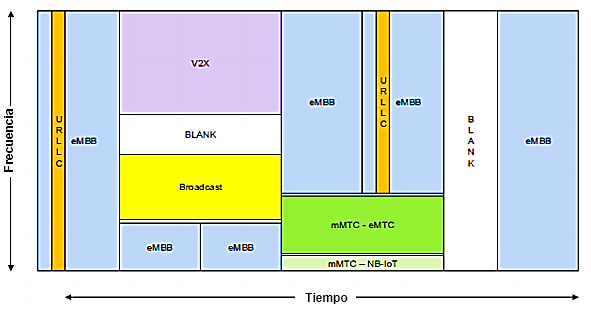
\includegraphics[scale=1]{5G NR soportará múltiples servicios con distintos requerimiento de QoS}
\decoRule
\caption[5G NR soportará múltiples servicios con distintos requerimiento de QoS]{5G NR soportará múltiples servicios con distintos requerimiento de QoS}
\label{fig:5gqos}
\end{figure}

%----------------------------------------------------------------------------------------
%	SECTION 
%----------------------------------------------------------------------------------------

\section{Análisis del estándar NB-IoT} \label{NBIoT}

El estándar NB-IoT fue especificado en el reporte TR 45.820 (\textit{release} 13) de la 3GPP \parencite{3GPP2019}. Sus parámetros fundamentales son:\newline

Para el enlace de subida (\textit{uplink}), como su nombre lo indica, tiene un ancho de banda estrecho de 180 kHz y un espacio de sub-portadora de 3.75 kHz (ancho de banda de transmisión mínimo para un dispositivo). Por lo tanto puede asignar 48 sub-portadoras [\textit{véase Figura~\ref{fig:NBIoT}}].

\begin{figure}[th]
\centering
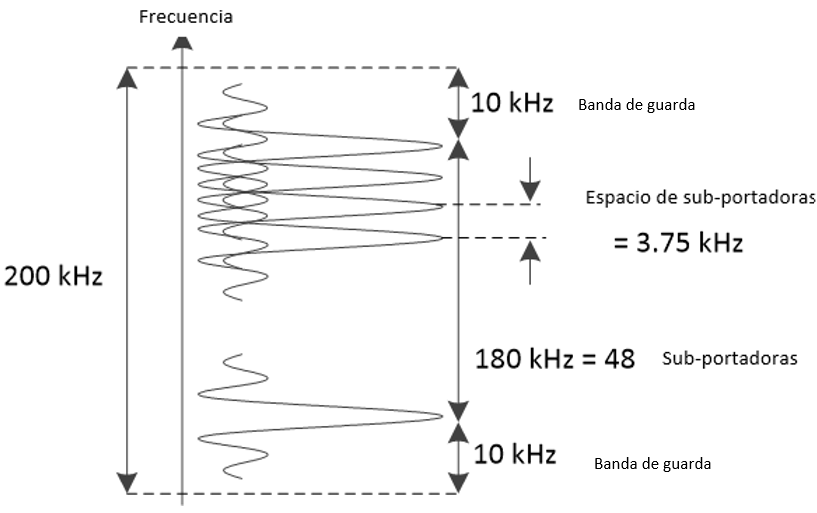
\includegraphics[scale=.7]{Estructura de ancho de banda y subportadoras en NB-IoT}
\decoRule
\caption[Estructura de ancho de banda y subportadoras en NB-IoT.]{Estructura de ancho de banda y subportadoras en NB-IoT.}
\label{fig:NBIoT}
\end{figure}

En el enlace de bajada (\textit{downlink}), se conserva la estructura de transmisión del enlace descendente de \textit{Long Term Evolution} (LTE) con un espaciado de sub-portadora de 15 kHz. Por lo tanto, NB-IoT puede proporcionar velocidades de datos de casi 250 kb / s en el enlace descendente y 20 kb / s en el enlace ascendente.\newline

Es preciso puntualizar que para lograr una mayor tasa de datos, de acuerdo con el Teorema de Shannon-Hartley (Ecuación~\ref{eqn:Shannon}), el ancho de banda debe ser elevado o se debe tener una relación S/N alta. Para el caso de NB-IoT se cuenta con un ancho de banda muy pequeño (3.75KHz), por lo cual alcanzar una buena relación S/N (S/I para sistemas celulares) es de suma importancia.\\

\subsection{Modos de operación}

NB-IoT puede implementarse como una portadora autónoma utilizando cualquier espectro disponible con un ancho de banda superior a 180 kHz. Esto se conoce como la implementación stand-alone. Un caso de uso de este despliegue autónomo es que un operador GSM despliegue NB-IoT en su banda GSM reajustando parte de su espectro \parencite{Liberg2018}.\newline


NB-IoT también está diseñado para su despliegue en las redes LTE existentes, ya sea utilizando uno de los bloques de recursos físicos (PRB) de LTE o utilizando la banda de guarda LTE.\newline

Para el modo de operación independiente y de banda de guarda, el PRB de enlace descendente y ascendente debe establecerse simétricamente y para el modo en banda, el despliegue del PRB estará restringido a algunos prefijos de PRB’s de acuerdo al ancho de banda LTE, (ya sea 3, 5, 10, 15 o 20 MHz.) esto debido a la sincronización entre el UE y la eNB \parencite{NBIoTDeploymentGSMA}.

\begin{figure}[th]
    \centering
    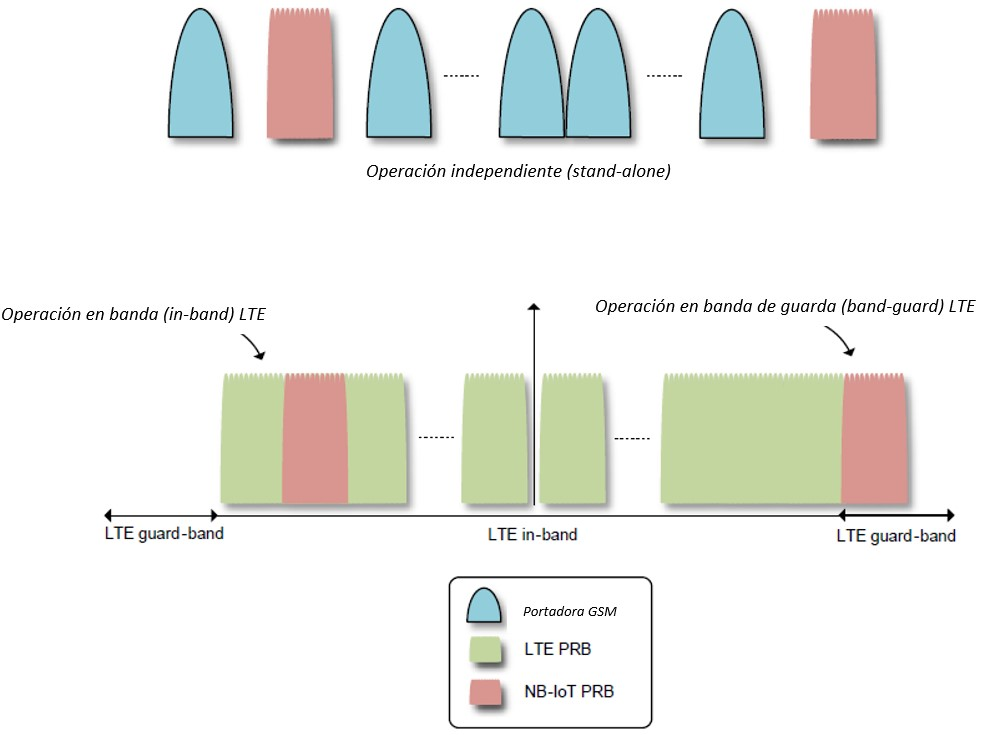
\includegraphics[scale=.5]{modooperacionNBIOT}
    \decoRule
    \caption[Modos de Operación en NB-IoT.]{Modos de Operación en NB-IoT. \parencite{Liberg2018}}
    \label{fig:NBIoT2}
\end{figure}


\subsection{Clases de Potencia}

Algunas aplicaciones de IoT son particularmente sensibles al consumo de energía. Para minimizar el impacto de la conectividad en la duración de la batería del dispositivo, en el \textit{release} 13, se determinó que los UE podrán usar dos opciones de clase de potencia. Uno es el nivel de potencia del dispositivo móvil LTE tradicional de \textbf{23dBm} (\textit{Power Class 3}) y uno nuevo, con menos potencia de salida, de \textbf{20dBm} (\textit{Power Class 5}). El \textit{release} 14 de 3GPP agrega una nueva clase de potencia aún menor, de \textbf{14dBm} (\textit{PowerClass 6}) \parencite{NBIoTDeploymentGSMA}.

\subsection{Modos de transmisión en enlace ascendente (UL) }
Existen dos modos de transmisión para el enlace UL, en el modo \textit{singletone} sólo se puede asignar una subportadora a cada dispositivo NB-IoT, por el contrario en el modo \textit{multitone}, la agregación de subportadoras es posible, esto con el fin de alcanzar una mayor tasa de transmisión \parencite{RohdeNB}. En \parencite{Shahini2019} se evaluó el uso \textit{multitone} en anchos de banda de subportadoras de 3.75 kHz, y es este escenario el que se evaluó en este trabajo puesto que permitiría dar servició a una mayor cantidad de dispositivos al mismo tiempo.\newline

Finalmente, se admiten los modos de \textit{singletone} y \textit{multitone}, cuando el PRB se divide en 12 subportadoras, cada una de ellas con un ancho de banda de 15 kHz. En \parencite{Mostafa2019} se estudió más a fondo el uso de \textit{singletone} y \textit{multitone} en transmisiones UL.\newline

\subsection{Características del tráfico NB-IoT}

En los Reportes autónomos móviles (MAR, \textit{Mobile Autonomous Reporting}) se definen cuatro tipos de paquetes diferentes:

\subsubsection{Informes de excepción}

Se espera que muchas aplicaciones de tipo sensor monitoreen una condición física y activen un informe de excepción cuando se detecte un evento en específico. Estos eventos serán, en general, raros y ocurrirán cada par de horas, pocos días o incluso meses. Ejemplos de tales paquetes incluyen los producidos por detectores de humo, notificaciones de fallas de energía de medidores inteligentes, notificaciones de manipulación, etc.\newline

\subsubsection{Informes periódicos}\label{Informesperiodicos}

Se espera que los informes periódicos de enlace ascendente sean comunes para aplicaciones de IoT celular como informes de medición de servicios inteligentes (gas / agua / electricidad), agricultura inteligente, entorno inteligente, etc. El modelo de tráfico de informes de enlace ascendente periódico MAR se utiliza en simulaciones a nivel de sistema para análisis de capacidad.\newline

El tamaño de la carga útil sigue una distribución de Pareto con parámetro $\alpha$ = 2.5 y tamaño mínimo de carga útil = 20 bytes con un corte en 200 bytes, es decir, las cargas superiores a 200 bytes serán limitadas a 200 bytes.\newline

Una vez revisadas estas clasificaciones de tráfico compatibles para NB-IoT, se asignaron los modelos de tamaño de paquete a los servicios seleccionados en la \textit{Tabla~\ref{tab:appssim}} de la sección anterior.\newline

La adición de la columna "Tamaños de paquete"  para la \textit{Tabla~\ref{tab:appssim}} se da en la \textit{Tabla~\ref{tab:trafpkt}}.
\begin{table}
\caption{Caracterización del tráfico de paquetes en aplicaciones seleccionadas para la simulación.}
\label{tab:trafpkt}
\centering
\begin{tabular}{*{2}{m{7cm}}}\\ 
\textbf{\textit{Servicio}} & \textbf{Tamaño de paquetes} \\ \hline \hline
\textit{Control de iluminación (Smart City) } & \footnotesize{ Activación aleatoria \textbf{UL}: 20 bytes \textit{payload} \textbf{DL}: ACK de 0 bytes } \\ \hline 
\textit{Monitoreo del consumo de agua y electricidad en la ciudad (Smart City) } & \footnotesize{ Activación periódica \textbf{UL}: distribución de Pareto con parámetro alfa = 2.5 y tamaño mínimo de carga útil de la aplicación = 20 bytes con un corte a 200 bytes \textbf{DL}: ACK de 0 bytes 50\% de las veces. } \\ \hline 
\textit{Detección de terremotos (Smart Environment)}  & \footnotesize{ Activación aleatoria \textbf{UL}: 20 bytes \textit{payload} \textbf{DL}: ACK de 0 bytes } \\ \hline 
\textit{Monitoreo de contaminación del aire (Smart Environment) } & \footnotesize{ Activación periódica \textbf{UL}: distribución de Pareto con parámetro alfa = 2.5 y tamaño mínimo de carga útil de la aplicación = 20 bytes con un corte a 200 bytes \textbf{DL}: ACK de 0 bytes 50\% de las veces. } \\ \hline 
\textit{Control dinámico de semáforos (Smart Transport and Mobility)}  & \footnotesize{ Activación aleatoria \textbf{UL}: distribución de Pareto con parámetro alfa = 2.5 y tamaño mínimo de carga útil de la aplicación = 20 bytes con un corte a 200 bytes \textbf{DL}: ACK de 0 bytes 50\% de las veces. } \\ \hline 
\textit{Otros dispositivos mMTC}  & \footnotesize{ Activación aleatoria \textbf{UL}: 20 bytes \textit{payload} \textbf{DL}: ACK de 0 bytes } \\  
\end{tabular}
\end{table}

\subsection{Indicadores clave de rendimiento (KPIs)}

Debido a que 5G representará un cambio radical a las generaciones anteriores, se puede prever que habrá nuevos indicadores de evaluación. El diseño de estos indicadores directamente medibles, por un lado, necesita combinar las características de los nuevos servicios, y por otro lado, debe aprender completamente de la experiencia de los KPI clásicos de generaciones anteriores como lo son: el \textit{throughput, }dada una probabilidad de salida y la latencia. Además la densidad de conexión, la densidad de volumen de tráfico y el consumo de energía son KPI's que preocupan también a las redes 5G/IoT \parencite{WirelessSim}.\newline

Para cumplir con el conjunto de requisitos de mMTC, NB-IoT debe admitir principalmente cuatro indicadores clave de rendimiento (KPI):

\begin{enumerate}
\item  Vida útil de la batería del dispositivo más allá de 10 años, suponiendo una capacidad de energía almacenada de 5 Wh.
\item  Densidad de conexión masiva de hasta 1M dispositivos por km cuadrado en un entorno urbano.
\item  Latencia de como máximo 10 s.
\item  Una tasa máxima alcanzable de hasta 200kbps (subida).
\end{enumerate}

De los KPIs antes enumerados este simulador obtuvo resultados acerca de la densidad de conexión masiva de dispositivos y de las tasas objetivo alcanzadas por estos.

\break
%----------------------------------------------------------------------------------------
%	SECTION 
%----------------------------------------------------------------------------------------

\section{Análisis de modelos para la evaluación de redes 5G/IoT}\label{AnalisisMODELOS}
Los modelos necesarios para caracterizar el comportamiento de redes móviles, desde el punto de vista de simulaciones a nivel de sistema, se presentan a continuación \parencite{WirelessSim}:
\begin{enumerate}
    \item  Modelo de despliegue de BSs y UEs.
    \item  Modelo de antenas (MIMO, MISO, entre otras) y formación de haz.
    \item  Modulación y codificación.
    \item  Modelo de canal.
    \item  Patrones de Movilidad.
    \item  Calendarizadores (planificadores de recursos).
    \item  Esquema de acceso múltiple al medio.
    \item  Modelos de tráfico.
\end{enumerate}


Los modelos que se incluyeron en el simulador se describen en las siguientes subsecciones:

\subsection{Modelo de despliegue de UEs}

Los modelos del posicionamiento de las estaciones base y los nodos IoT utilizan diferentes estrategias de despliegue (como se puede ver en la \textit{Figura~\ref{fig:BSs}}). Este aspecto, como los demás, es de mayor o menor importancia dependiendo de los objetivos de la simulación, es decir, para un alcance comercial resulta importante simular el despliegue determinístico de los actores de la red. Por otro lado para un alcance con fines de análisis en el diseño y dimensionamiento de estas redes resulta más adecuado un despliegue aleatorio. \newline

Diversos autores coinciden en que varias distribuciones de redes móviles siguen un proceso estocástico \parencite{Kouzayha2018}\parencite{Zhang2017}. La geometría estocástica es una rama de la probabilidad con muchas aplicaciones que permiten el estudio de fenómenos aleatorios en el plano o en dimensiones superiores \parencite{Haenggi2009}. Recientemente se ha utilizado con éxito para modelar la distribución espacial de células pequeñas como las femtoceldas \parencite{TurjmanSmallCells}. \newline

En este proyecto con fines de diseño y análisis, se simularon ambos despliegues, uno uniforme y otro siguiendo una geometría estocástica, es decir, un PPP.

\subsection{Modelo de canal}

Un buen diseño de sistema necesitó de conocer las características del canal de propagación a través de las frecuencias de microondas y ondas milimétricas. \newline

Los modelos de canal son necesarios para simular la propagación de una manera reproducible y rentable, y se utilizan para diseñar y comparar con precisión las interfaces de radio y el despliegue del sistema. Los parámetros comunes del modelo de canal inalámbrico incluyen frecuencia de portadora, ancho de banda, distancia entre el transmisor (Tx) y el receptor (Rx), los efectos ambientales y otros requisitos necesarios. El desafío definitivo para un modelo de canal 5G es proporcionar una base física fundamental, a la vez flexible y precisa, especialmente en un amplio rango de frecuencias como 0.5--100 GHz \parencite{Rappaport2017}. Los modelos de canal investigados se dividen principalmente de acuerdo al escenario en el que se están diseñando, ya sea \textit{Urban Macro (UMa) o Urban Micro (UMi)}, además de la condición del ambiente si es que hay línea de vista (\textit{LoS}) entre el UE y la BS.\newline

Existe una gama amplia de modelos de canal propuestos para redes 5G, (p.ej. 3GPP, WINNER I/II, QuaDRiga/ mmMagic, 5GCM, METIS, MiWEBA, IEEE \parencite{WirelessSim}). Aunque existen diversos modelos, los modelos de canal 3GPP y WINNER II son los más conocidos y empleados en la industria de comunicaciones móviles \parencite{Sun2016}, conteniendo una gran diversidad de escenarios de despliegue como lo son \textit{UMi, UMa, indoor office (InH)}, etc. Además proveen parámetros clave del canal incluyendo probabilidades de línea de vista (\textit{LoS}), modelos de pérdida por trayectoria, retardos y niveles de potencia por trayectoria \parencite{Sun2016}. \newline

El modelo implementado se trató de uno teórico y estocástico, en vez de uno empírico, ya que este proyecto está enfocado en el teletráfico. Los modelos empíricos suelen ser más sofisticados y piden una gran cantidad de parámetros de entrada. Por lo tanto se eligieron modelos estocásticos que se adaptaran al rango de frecuencia de transmisión y a los ambientes urbanos que se propusieron.\newline

En \parencite{Sun2016}, los autores evaluaron tres diferentes modelos de propagación estocásticos de perdida por trayectoria a larga escala para ser implementados a través de la banda de frecuencias de microondas y ondas milimétricas. ABG, CI y CIF son modelos estadísticos de propagación para multi-frecuencias (estocásticos) que describen los parámetros de larga escala con pérdida de trayectoria de acuerdo a la distancia.

Los modelos evaluados fueron: 
\begin{enumerate}
\item  ABG: Modelo Alpha-Beta-Gamma.
\item  CI: Modelo de pérdida por trayectoria de distancia de referencia de espacio libre cercano.
\item  CIF: Modelo CI con un exponente de pérdida de trayectoria ponderado en frecuencia.
\end{enumerate}

\begin{flushleft}
 Para el primero, la ecuación del modelo ABG está dada por:
 \begin{equation}
    L^{ABG}_p(f,d)_{\left[dB\right]}=10 \alpha {\ log}_{10}\left(\frac{d}{1m}\right)+\beta +\ 10\gamma {\ log}_{10}\left(\frac{f}{1GHz}\right)+\ x^{ABG}_{\sigma .}, donde\ d\ge 1m
    \label{eqn:ABG}
\end{equation}
\[\alpha \to coeficiente\ que\ representa\ la\ dependencia\ de\ la\ perdida\ por\ trayectoria\ con\ la\ distancia\] 
\[\gamma \to coeficiente\ que\ representa\ la\ dependencia\ de\ la\ perdida\ por\ trayectoria\ con\ la\ frecuencia\] 
\[\beta \to es\ un\ valor\ de\ compensación\ para\ la\ pérdida\ por\ trayectoria\ (en\ dB's)\] 
\[x^{ABG}_{\sigma .}\to es\ una\ variable\ aleatoria\ gaussiana\ de\ media\ cero\ con\ una\ desviaci\textrm{ó}n\ est\textrm{á}ndar \]
\[sigma \ [dB], que\ describe\ las\ fluctuaciones\ de\ se\textrm{ñ}al\ a\ gran\ escala\ (es\ decir,\ ensombrecimiento)\]

Para el segundo, la ecuación del modelo CI está dada por:
\begin{equation}
    L^{CI}_p(f,d)_{\left[dB\right]}=32.4+\ 10\ n{\ log}_{10}\left(\frac{d}{d_0}\right)+{\ 20\ log}_{10}\left(d_0\right)+{20\ log}_{10}\left(f\right)+x^{CI}_{\sigma .}, donde\ d\ge d_0
    \label{eqn:CI}
\end{equation}
\[x^{CI}_{\sigma .}\to es\ una\ variable\ aleatoria\ gaussiana\ de\ media\ cero\ con\ una\ desviaci\textrm{ó}n\ est\textrm{á}ndar \]
\[sigma \ [dB], que\ describe\ las\ fluctuaciones\ de\ se\textrm{ñ}al\ a\ gran\ escala\ (es\ decir,\ ensombrecimiento)\]

Para el tercero, la ecuación del modelo CIF está dada por:
\begin{equation}
    L^{CIF}_p(f,d)_{\left[dB\right]}=32.4+\ 10\ n{\left(1+b \left(\frac{f-f_0}{f_0}\right) \right)log}_{10}\left(d\right)+{20\ log}_{10}\left(f\right)+x^{CIF}_{\sigma .},  donde\ d\ge 1m
    \label{eqn:CIF}
\end{equation}
\[x^{CIF}_{\sigma .}\to es\ una\ variable\ aleatoria\ gaussiana\ de\ media\ cero\ con\ una\ desviaci\textrm{ó}n\ est\textrm{á}ndar  \]
\[ sigma \ [dB], que\ describe\ las\ fluctuaciones\ de\ se\textrm{ñ}al\ a\ gran\ escala\ (es\ decir,\ ensombrecimiento)\]
\end{flushleft}

Cada uno de estos modelos han sido recientemente estudiados por organizaciones de estandarización como 3GPP y son propuestos para su uso en el diseño de sistemas inalámbricos de comunicación de 5G enfocados en escenarios \textit{UMa, UMi, InH,y SM}.\newline

De acuerdo al análisis de sensibilidad en \parencite{Sun2016}, se demostró que el modelo CI es el más adecuado para entornos al aire libre debido a su precisión, simplicidad y rendimiento de sensibilidad, dado que la pérdida de trayectoria medida depende poco de la frecuencia en ambientes exteriores más allá del primer metro de propagación de espacio libre.\newline

Por otro lado, el modelo CIF es muy adecuado para entornos interiores, ya que proporciona una desviación estándar más pequeña que el modelo ABG en muchos casos, incluso con menos parámetros del modelo y tiene una precisión superior cuando se analiza con el análisis de sensibilidad.\newline

Los modelos CI y CIF son más robustos y precisos en comparación con el modelo ABG, por lo que es confiable la aplicación del modelo CI para simular entornos en exteriores y el CIF para interiores \parencite{Sun2016}.\newline

De acuerdo a lo propuesto en la \textit{sección~\ref{AppsEscenario} }, el ambiente macro urbano (UMa) que consideramos está dirigido a un entorno en exteriores. Por lo que se seleccionó al modelo CI (Modelo de pérdida por trayectoria de distancia de referencia de espacio libre cercano). \newline

Los parámetros que requiere este modelo (\textit{Ecuación~\ref{eqn:CI}}) son: la distancia entre la BS y el UE, la frecuencia fundamental de operación y una variable aleatoria de media cero con una desviación estándar $\sigma$ [dB], que describirá las fluctuaciones de señal a gran escala (es decir, ensombrecimiento[\textit{shadowing}]).\newline

Sin embargo, para este modelo de canal no se implementaron las pérdidas por ensombrecimiento, se optó por incorporar las perdidas por multitrayectoria (\textit{multipath}) ya que en el caso del estándar NB-IoT, que usa anchos de banda pequeños, se espera que sea suceptible a las variaciones rápidas del canal. Por lo tanto, en lugar de utilizar la variable aleatoria gaussiana propia del modelo, se implementó el desvanecimiento rápido incorporando una variable aleatoria tipo Rayleigh.\newline

Por último, los autores proponen a $d_{0} = 1 m$ en los modelos de pérdida por trayectoria para sistemas 5G ya que se espera que las distancias de cobertura serán más cortas a frecuencias más altas. Además, lo que se espera son futuras celdas pequeñas, es probable que las BS se monten más cerca de las obstrucciones. La estandarización a una distancia de referencia de 1 m simplifica las comparaciones de mediciones y modelos y proporciona una definición estándar para el PLE, al tiempo que permite la intuición y el cálculo rápido de la pérdida de trayectoria.

\subsection{Esquema de acceso múltiple al medio}

\subsubsection{Acceso Múltiple No Ortogonal (NOMA)}\label{NOMA_C4}

Se estudió en la Sección~\ref{NOMA_C2}, el uso de NOMA y su soporte eficientemente de conectividad masiva. El diseño de NOMA en transmisiones de subida (\textit{uplink}) ha sido propuesto en \parencite{Al-Imari2014} y el diseño óptimo de NOMA en transmisiones de bajada (\textit{downlink}) ha sido propuesto en \parencite{Zhu2019}.\newline

En \parencite{Zhang2017} se implementó NOMA emparejando selectivamente dos usuarios, es decir, se escogía a un usuario con una condición de canal muy buena (cerca de la BS) y otro con una condición de canal muy pobre (en el borde de la celda). Por otro lado en \parencite{Shahini2019}, se implementó NOMA usando la técnica de agrupamiento de usuarios, considerando un entorno donde conviven dispositivos mMTC y URLLC (estos tienen mayores requisitos de tasa en comparación con los dispositivos mMTC), de igual manera se agrupan con otros usuarios (p.ej., 2, 3 o 4 usuarios) de diferente tipo (mMTC y URLLC) y se ordenan convenientemente para implementar SIC.\newline

NB-IoT no es capaz de proveer conectividad a una cantidad masiva de dispositivos IoT como se espera en el futuro, así para el diseño se consideró la metodologia en \parencite{Shahini2019}, donde los dispositivos activos de URLLC y mMTC comparten un PRB para la transmisión de datos en el enlace ascendente. El ancho de banda disponible se divide en un conjunto de frecuencias (subcanales) $S$. De hecho, el ancho de banda del sistema se puede dividir por igual en 48 o 12 subportadoras en los sistemas NB-IoT. La relación de la distribución de dispositivos mMTC con los URLLC se fijó a 3 a 1. Todo esto con base en las consideraciones del modelo de sistema en \parencite{Shahini2019}.\newline

En \parencite{Shahini2019}, se utiliza la nomenclatura que se enlista a continuación para desarrollar su propuesta, misma que se utilizó en este documento:\label{VariablesSHahini}

\begin{itemize}
    \item U: Lista de dispositivos uRLLC
    \item M: Lista de dispositivoss mMTC
    \item S: Lista de Subportadoras s
    \item C: Lista de Grupos NOMA
    \item $k_{max}$ Rango máximo de usuarios en un grupo NOMA
    \item $R_{m}^{th}:$ Tasa objetivo del enésimo dispositivo m mMTC 
    \item $R_{u}^{th}:$ Tasa objetivo del enésimo dispositivo u uRLLC
    \item $P_{m}^{max}:$ Potencia máxima del enésimo dispositivo m mMTC 
    \item $P_{u}^{max}:$ Potencia máxima del enésimo dispositivo u uRLLC (i.e. 23dBm)
    \item $P_{m}^{s}:$ Potencia del enésimo dispositivo m mMTC 
    \item $P_{u}^{s}:$ Potencia del enésimo dispositivo u uRLLC 
    \item $h_{m}^{s}:$ Ganancia de canal del enésimo dispositivo m mMTC sobre la portadora s
    \item $h_{u}^{s}:$ Ganancia de canal del enésimo dispositivo u uRLLC sobre la portadora s
    \item ${\hat S}$: Lista de subportadoras asignadas
    \item $S_{a}^{c}$: Lista de subportadoras asignadas al enésimo cluster
    \item ${C_{ns}}$: Lista de cluster aún no asignados
    \item $W$ Ancho de banda en un tono NB-IoT (3.75KHz)
    \item $\alpha$, $\gamma$, $\beta$ son variables binarias que indican asignaciones.
\end{itemize}

La tasa de datos alcanzable por un dispositivo $m$ (mMTC) en términos de la tasa agregada sobre las subportadoras asignadas se puede expresar como \parencite{Shahini2019}:
\begin{equation}
{R_{m}}=\sum \limits _{c \in \mathcal {C}} {\sum \limits _{k \in \mathcal {K}} {\alpha _{m}^{c,k}\sum \limits _{s \in \mathcal {S}} {{\gamma ^{s,c}}W} } } \times {\log _{2}}\left ({{1 + \frac {{{{\left |{ {h_{m}^{s}} }\right |}^{2}}p_{m}^{s}}}{{N_{0}W + \sum \limits _{d \in \mathcal {M}\backslash m} {\sum \limits _{h = k + 1}^{{k_{\max }}} {\alpha _{d}^{c,h}{{\left |{ {h_{d}^{s}} }\right |}^{2}}p_{d}^{s}} } }}} }\right)
\label{eqn:Rm}
\end{equation}

Del mismo modo, la Tasa de datos alcanzable por un dispositivo $u$ (URLLC) puede determinarse mediante el teorema de Shannon-Hartley. Hay que tomar en cuenta que los rangos de URLLC siempre son mayores que los de mMTC en cada clúster NOMA. Por lo tanto, reciben interferencia de todos los miembros del clúster mMTC, así como de los miembros del clúster URLLC con rangos más altos. 
Por lo tanto, la tasa de datos alcanzable de un dispositivo $u$ URLLC sobre las subportadoras asignadas es \parencite{Shahini2019}:
\begin{equation}
{R_{u}}=\sum \limits _{c \in \mathcal {C}} {\sum \limits _{k \in \mathcal {K}} {\beta _{u}^{c,k}\sum \limits _{s \in \mathcal {S}} {{\gamma ^{s,c}}W} } } \times {\log _{2}}\left ({{1 + \frac {{{{\left |{ {h_{u}^{s}} }\right |}^{2}}p_{u}^{s}}}{{N_{0}W + \sum \limits _{d \in \mathcal {U}\backslash u} {\sum \limits _{h = k + 1}^{{k_{\max }}} {\beta _{d}^{c,h}{{\left |{ {h_{d}^{s}} }\right |}^{2}}p_{d}^{s}}} \sum \limits _{m \in \mathcal {M}} {\sum \limits _{h = k + 1}^{{k_{\max }}} {\alpha _{d}^{c,h}{{\left |{ {h_{m}^{s}} }\right |}^{2}}p_{m}^{s}} } }}} }\right)
\label{eqn:Ru}
\end{equation}

\subsection{Modelos de tráfico}

Los modelos de tráfico en comunicaciones móviles buscan acercarse, lo más posible a cómo transmiten datos o realizan peticiones de acceso los dispositivos que intentan modelar. Estos modelos de tráfico pueden clasificarse en modelos de tráfico\textbf{agregado } y modelos de tráfico \textbf{fuente} \parencite{Laner2013}. El tráfico agregado simula un flujo de tráfico que se agrupa para recibir un tratamiento común, mientras que en los modelos de tráfico fuente es justamente cada una de las fuentes generadoras del tráfico la que se simula y frecuentemente se hace acompañada de una cadena de Markov que intenta representar los distintos estados del dispositivo fuente y la probabilidad de transición entre ellos.\newline

Sin importar el modelo de tráfico a utilizar, en \parencite{Laner2013} se señala que los modelos de tráfico que pretendan simular el comportamiento de dispositivos de MTC (\textit{Machine Type Communications}) deben:

\begin{itemize}
\item  Capturar con precisión el comportamiento de un solo dispositivo de MTC 
\item  Permitir la simulación concurrente de una cantidad masiva de dispositivos con su potencial reacción síncrona a un evento.
\end{itemize}

Antes de elegir un modelo es importante conocer las propiedades del tráfico máquina a máquina (M2M, \textit{Machine to Machine}), el cual se considera una forma de transmisión de datos que no requiere necesariamente de la interacción humana (ETSI, 2010) y corresponde justamente al tráfico de los nodos IoT, de \parencite{Laner2013} se tiene:

\begin{itemize}
\item  Cantidad masiva de dispositivos
\item  Pocos paquetes de un tamaño pequeño a ser transmitidos por dispositivo
\item  Periodos largos entre dos transmisiones consecutivas
\item  Tráfico de subida (\textit{uplink)} dominante
\item  Transmisiones en tiempo real y transmisiones tolerantes al retraso
\item  Paquetes no sincronizados y paquetes sincronizados
\item  Activación de tráfico que depende del espacio y tiempo
\end{itemize}

Además, se hace  la distinción de 3 patrones de tráfico que pueden presentarse en estos dispositivos:

\begin{enumerate}
    \item \underbar{Actualización periódica (PU, }\textit{\underbar{Periodic Update}}\underbar{):} Este tipo de tráfico ocurre cuando el dispositivo transmite reportes de estado y/o actualizaciones de estado de manera periódica. Puede verse como una activación por evento que ocurre por el mismo dispositivo en un intervalo periódico. Típicamente, el tráfico PU no necesita transmitirse en tiempo real y cuenta además de un patrón periódico de tiempo con un tamaño constante en sus paquetes. Un ejemplo típico de estos dispositivos son medidores inteligentes (por ejemplo gas, electricidad, agua).
    \item \underbar{Activación por evento (ED, }\textit{\underbar{Event-Driven}}\underbar{):} En caso de que un evento desencadene la transmisión de datos de un dispositivo, el patrón de tráfico corresponde a esta segunda clase. Un evento puede ser causado ya sea por la medición de un parámetro que sobrepasó un límite y activó alguna alarma o bien por el nodo que actúa como servidor y envía comandos al dispositivo. El tráfico \textit{Event-Driven} puede requerir ser transmitido tanto en tiempo real o no, un ejemplo de mensajes de subida que debieran ser transmitidos en tiempo real son alarmas y notificaciones médicas de emergencia, en cuanto a los mensajes de bajada, estos podrían ser la distribución de mensajes de emergencia locales, por ejemplo en caso de sismo o tsunamis. En algunos casos, como ya se mencionó, este tráfico no necesita ser transmitido en tiempo real. Por ejemplo, cuando un dispositivo IoT envía una actualización de su ubicación al servidor o se reciba una actualización de \textit{firmware }desde este.
    \item \underbar{Intercambio de carga útil (PE, }\textit{\underbar{Payload Exchange}}\underbar{):} este último tipo de tráfico ocurre después de una transmisión previa (PU o ED). Comprende todos los casos en los que es necesario un mayor intercambio de datos entre el dispositivo que envía y su servidor, este tráfico se espera sea predominantemente de subida y puede ser de tamaño constante o variable según la aplicación.
\end{enumerate}

Las aplicaciones en el mundo real que brindan servico a dispositivos de IoT generarán casi siempre tráfico en una combinación de estos tipos, más un estado de reposo o de ahorro de batería. Este simulador como se verá en la sección \ref{Chapter5} generó tráfico únicamente de los tipos: Actualización periódica y Activación por evento.\newline
\begin{figure}[th]
\centering
\includegraphics[scale=1]{Figures/Estructura de los estados principales del tráfico M2M}
\decoRule
\caption[Estructura de los estados principales del tráfico M2M]{Estructura de los estados principales del tráfico M2M}
\label{fig:}
\end{figure}

Ahora se presentan los modelos de tráfico más recurrentes para la simulación de comunicaciones M2M.

\subsubsection{Modelos de tráfico agregado}

Han sido propuestos por la 3GPP al reconocer la importancia de caracterizar el tráfico M2M. Se trata en realidad de 2 modelos de tráfico agregado generado por una gran cantidad de usuarios, el primero modela el tráfico generado de forma aleatoria y el segundo modela tráfico síncrono en el tiempo, esto se puede observar en la \textit{Tabla~\ref{tab:trafico3gpp}}.

\begin{itemize}
\item  \textit{Modelo 1} - Modelo de tráfico agregado sin correlación 3GPP: Genera tráfico sin correlación en un intervalo específico de tiempo. Lo que significa que no se tomarían en cuenta la correlación entre los dispositivos IoT. Utiliza una distribución uniforme para modelar el tráfico agregado en un intervalo de tiempo específico.
\item  \textit{Modelo 2 -} Modelo de tráfico agregado con correlación 3GPP: Este modelo genera tráfico correlacionado en un intervalo de tiempo, asumiendo que todas las máquinas se encuentran sincronizadas. Utiliza una distribución beta para modelar en tráfico agregado en un intervalo de tiempo específico.
\end{itemize}

\begin{table}
\caption{Modelos de tráfico agregado propuestos por la 3GPP para comunicaciones M2M}
\label{tab:trafico3gpp}
\centering
\begin{tabular}{*{2}{m{8.5cm}}}\\
\textbf{Sincronizado/Coordinado/Correlacionado\newline (En un intervalo limitado en el tiempo)} & \textbf{No sincronizado/No coordinado/ No correlacionado\newline (En un intervalo limitado en el tiempo)} \\ \hline \hline
Distribución de probabilidad de arribo de paquetes/peticiones f(t) en [0,1] : \underbar{Beta} (3,4) & Distribución de probabilidad de arribo de paquetes/peticiones f(t) en [0,1]: \underbar{Uniforme} \\ 
Número de dispositivos: 1 000, 3 000, 5 000, 10 000, 30 000. & Número de dispositivos: 1 000, 3 000, 5 000, 10 000, 30 000. \\ 
Periodo \textit{T }: 10 s & Periodo \textit{T }: 60 s \\ 
\end{tabular}
\end{table}

La principal ventaja de los modelos de tráfico agregado es su fácil implementación (en términos de una baja complejidad computacional) cuando se simulan una gran cantidad de dispositivos. Por otro lado, como se menciona en \parencite{IoTTrafficHossfeld}, la imprecisión de estos modelos para reflejar el comportamiento real del sistema es su principal desventaja.

\subsubsection{Modelos de tráfico fuente}

Los modelos de tráfico fuente, modelan justamente el tráfico que genera cada uno de los dispositivos. Este tipo de modelado es más preciso que el de tráfico agregado ya que modela el comportamiento de cada nodo, sin embargo, puede  volverse muy complejo cuando se agrega una gran cantidad de dispositivos (fuentes) y comportamientos. A continuación se presentan y analizan dos modelos de tráfico fuente.

\begin{itemize}
\item  \textit{Modelo 3:} Modelo de fuente de \textit{Semi-Markov} (\textit{Semi-Markov Models, SMM)}

En este modelo de fuente cada dispositivo se modela utilizando una cadena de Markov en la que se define la probabilidad de transición entre estados. Los estados que se encontrarán casi siempre modelados son los mencionados anteriormente: el de actualización periódica (PU), el de activación por evento (ED) y el de intercambio de carga útil. La \textit{Figura~\ref{fig:SMM}} muestra cómo se verían modelados los estados de un dispositivo en una cadena de Markov.\newline

La probabilidad de transición entre el mismo estado es 0, además los tiempos de espera y la longitud de los mensajes son generados de acuerdo a una distribución de probabilidad que es independiente de cada estado y potencialmente distinta para cada uno de ellos \parencite{IoTTrafficHossfeld}.\newline

\begin{figure}[th]
\centering
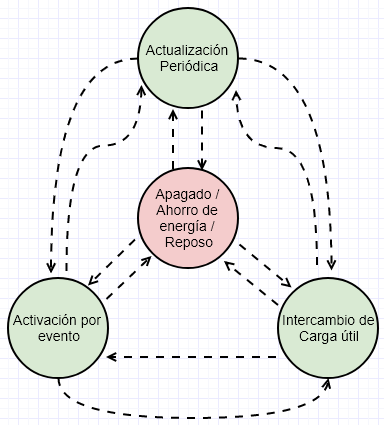
\includegraphics[scale=1]{Figures/Cadena de Markov del modelo SMM}
\decoRule
\caption[Cadena de Markov del modelo SMM]{Cadena de Markov del modelo SMM}
\label{fig:SMM}
\end{figure}

La principal ventaja del modelo de tráfico fuente SMM es que permitiría una descripción más detallada del comportamiento de los dispositivos IoT de manera individual, sin embargo no es capaz de capturar la relación que existe entre dos dispositivos cercanos que pudieran tener una cierta sincronía. Otra desventaja es que la complejidad del sistema aumenta considerablemente entre más dispositivos se simulan a diferencia de los modelos de tráfico agregado.

\item  \textit{Modelo 4:} Modelo de fuente de Procesos de Poisson emparejados Markov-modulados (CMMPP\textit{, Coupled Markov Modulated Poisson Process)}

En el modelo de tráfico CMMPP cada dispositivo MTC es representado como una entidad por separado y a diferencia del modelo SMM sí puede representarse una sincronización espacial y temporal entre dispositivos similares. La clave en el diseño del modelo CMMPP se presenta en encontrar un balance entre el emparejamiento entre distintos dispositivos y una complejidad tolerable del sistema cuando se tiene una gran cantidad de dispositivos \parencite{Gupta2018}.

Los procesos de Poisson Modulados con Markov (\textit{Markov modulated Poisson processes, MMPP}) consisten en procesos de Poisson que son modulados por la tasa $\lambda_{i[t]}$, que viene determinada por el estado de una cadena de Markov $sn[t]$. este principio se ve presentado en la \textit{Figura~\ref{fig:CMMPP}} donde \textit{p${}_{i,j}$}${}_{\ }$son las probabilidades de transición entre los estados de la cadena. En este modelo cada dispositivo \textit{n} del total\textit{ N} se encuentra representado por una cadena de Markov y un correspondiente proceso de Poisson. Debido a que existe una alta correlación en el cambio de estados de distintos dispositivos, tanto en el espacio como en el tiempo, es necesario realizar un emparejamiento. En los modelos genéricos, el emparejamiento se realiza introduciendo enlaces bidireccionales entre los dispositivos, pero esto sería sin lugar a dudas muy complejo de simular, de manera que en \parencite{Gupta2018} se propone un proceso de fondo actuando como \textit{maestro} el cual modula todos los dispositivos del mismo tipo.

\begin{figure}[th]
\centering
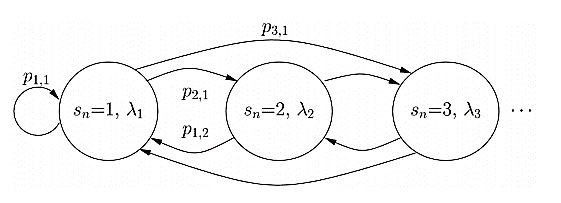
\includegraphics[scale=1]{Figures/Modelo MMPP en dispositivos MTC}
\decoRule
\caption[Modelo CMMPP en dispositivos MTC]{Modelo CMMPP: cada dispositivo MTC n está representado por una cadena de Markov con estados sn, que establecen el parámetro $\lambda$. Este parámetro es el promedio de la tasa de arribos, el cual modela el respectivo proceso de Poisson}
\label{fig:CMMPP}
\end{figure}

\end{itemize}

La principal ventaja como ya se mencionó del tráfico fuente frente al tráfico agregado es su precisión, por otra parte, la del tráfico agregado es su fácil implementación para un gran número de dispositivos. El modelo CMMPP es un intermedio entre estos dos casos, es decir mantiene la precisión del modelado de tráfico fuente mientras se mantiene la viabilidad para un gran número de máquinas. A continuación se presenta en la \textit{Tabla~\ref{tab:Traficos}} una comparación entre los distintos modelos mencionados.\newline
\begin{table}
\caption{Comparativa entre los modelos de tráfico MTC abordados}
\label{tab:Traficos}
\centering
\begin{tabular}{|p{3in}|p{1in}|p{0.8in}|p{1in}|} \\  \hline \hline
\textbf{\textit{Métrica}} & \textbf{Agregado~} & \textbf{SMM} & \textbf{CMMPP} \\ \hline 
\textit{Modelado de los dispositivos} &  & \checkmark & \checkmark \\ \hline 
\textit{Modelado de dispositivos coordinados} & \checkmark &  & \checkmark \\ \hline 
\textit{Coordinación espacial y temporal} &  &  & \checkmark \\ \hline 
\textit{Modelado de los paquetes} &  & \checkmark &  \\ \hline 
\textit{Modelado de la tasa de arribo} & \checkmark & \checkmark & \checkmark \\ \hline 
\textit{Tiempo de ejecución aleatorio factible} &  & \checkmark & \checkmark \\ \hline 
\textit{Ubicación del dispositivo} &  & \checkmark & \checkmark \\ \hline 
\textit{Emparejamiento de estados} &  &  & \checkmark \\ \hline 
\textit{Complejidad (N número de dispositivos)} & O(1) & O(N) & O(N) \\  
\end{tabular}
\end{table}

Como puede observarse en la \textit{Tabla~\ref{tab:Traficos}}, el modelo CMMPP es bastante conveniente a la hora de generar tráfico de dispositivos mIoT, pues este es capaz de simular la relación espacial y temporal que existiría entre los nodos. Si se regresa a la \textit{Tabla~\ref{tab:appssim}}, en la que se presentan los servicios que se simularán, se encuentra que servicios como el monitoreo de la condición del aire en la ciudad, la detección de terremotos, la manipulación de la iluminación y demás tendrán un comportamiento similar en un espacio limitado. De manera que el modelo CMMPP se seleccionó para la simulación de este sistema, complementándolo con un modelo determinístico para las aplicaciones que sólo producen tráfico periódico.\newline

Una explicación resumida del modelado  de tráfico fuente CMMPP se realiza a continuación \parencite{Gupta2018}:

\begin{enumerate}
\item  Un conjunto de \textit{k }estados se definen, cada uno asociado con una tasa de generación de paquetes ${\lambda }_k$. Un dispositivo IoT se encuentra en todo momento en algún de estos estados representados en una cadena de Markov formada por los estados antes mencionados.
\item  La transición entre los \textit{k} estados para cualquier dispositivo está definida por una matriz de probabilidad de cambio de estado $P_n$ ,la cual es a su vez una función de dos matrices de transición $P_u$ y $P_c$ ( que modelan el comportamiento no coordinado/no sincronizado y comportamiento coordinado/sincronizado respectivamente).
\item  Un factor de correlación espacial ${\delta }_n$ se asigna a cada dispositivo \textit{n. }Esto modela qué tanto se involucra un dispositivo durante la generación de tráfico coordinado en la red y dicta efectivamente la contribución de $P_c$ en la matriz resultante de probabilidad de transición de ese dispositivo.
\item  Se define un proceso $\mathit{\Theta}\left(t\right)$ el cual controla la matriz de  transición instantánea de estado del \textit{n-ésimo}\textbf{\textit{ }}dispositivo en el instante \textit{t.}
\end{enumerate}